\documentclass[10pt]{ctexart}
\usepackage[utf8]{inputenc}
\usepackage{geometry}
\geometry{left=2.2cm,right=2.2cm,top=2.3cm,bottom=2.3cm}
\usepackage{graphicx}
\usepackage{amsmath,amsfonts}
\usepackage{booktabs}
\usepackage{algorithm}
\usepackage{algorithmic}
\usepackage{caption}
\usepackage{subcaption}
\usepackage[compact]{titlesec}
\usepackage{setspace}
\usepackage{xcolor}

\setstretch{0.97}
\titlespacing*{\section}{0pt}{1.2ex plus 0.2ex minus .1ex}{0.8ex plus .1ex}
\titlespacing*{\subsection}{0pt}{1ex plus 0.1ex minus .1ex}{0.5ex plus .1ex}

\captionsetup{font=small,skip=4pt}

\begin{document}

\begin{center}
    {\Large\bfseries 多城物流联合库存与路径优化研究——以美团生鲜为例}\\*[0.8em]
    % {\normalsize \textit{美团物流优化团队}}\\*[0.3em]
    {\small 2026年4月}
\end{center}

\begin{abstract}
\noindent\textbf{摘要——}
生鲜电商的“最后一公里”配送网络面临着库存持有成本与运输成本之间的根本性权衡。本文针对一个由1个中央配送中心（CDC）和5个卫星城（共25个零售站点）组成的物流网络，提出了库存与路径联合优化框架。对每个城市，我们通过平衡仓储与运输成本来优化补货周期$T$；进而枚举全部$7^5=16{,}807$种全局$T$组合，以确定系统层面的最优解。最优配置实现了\textbf{24,874元/天}的总成本，各城市的最优补货周期从$T^*=1$到$T^*=6$不等。与统一$T$基线策略相比，差异化的最优策略最多可节省\textbf{20,058元/天}（80.6\%）。结果表明，在城市特征异质化的物流网络中，城市专属的补货政策对于成本高效运营至关重要。
\end{abstract}

\section{引言}
以美团为代表的生鲜电商平台每天都面临着将易腐商品从中央配送中心（CDC）补货至多个城市 hub，再分发到各个零售站点的挑战。补货周期$T$越长，长途运输频次越低，但平均库存水平和持有成本随之上升；反之，缩短$T$可降低仓储费用，却导致运输支出增加。现有实践往往将库存决策与路径决策割裂处理，或在所有城市强制采用统一的$T$，这常常导致次优结果。

本文针对美团的实际物流网络回答以下两个问题：
\begin{enumerate}
    \item \textit{城市层面}：每个城市的最优补货周期$T^*$是多少？仓储与运输成本如何相互作用？
    \item \textit{系统层面}：相对于各城市独立优化以及统一$T$策略，全局联合优化能带来多少额外价值？
\end{enumerate}

\section{问题描述}
网络由1个CDC和5个城市hub（A--E）组成。每个hub服务一组具有已知日需求的零售站点，且已知各城市到CDC的距离。有两种车型可供选择：大车（满载20万件）和小车（满载8万件）。规划目标是最小化\emph{日均总成本}，包括：（i）城市hub的库存持有成本；（ii）日均运输成本，含CDC到城市的长途运输以及城市内部到站点的末端配送。

决策变量为每个城市$i \in \{A,\dots,E\}$的整数补货周期$T_i \in \{1,\dots,7\}$，以及满足每次补货运力约束的车辆路径方案。

\section{方法论}
\subsection{城市级库存—运输模型}
对于给定城市和候选周期$T$，日均总成本为
\begin{equation}
    C(T) = C_s(T) + C_t(T),
\end{equation}
其中仓储成本与周期长度和日需求$d$成正比：
\begin{equation}
    C_s(T) = h \cdot \frac{T \cdot d}{2},
\end{equation}
$h$为单位持有成本。运输成本包含两部分：CDC到城市的长途固定成本（每次发车成本除以$T$摊销）以及城市内部的末端路径成本。末端路径问题通过穷举分组求解：我们将站点划分为每组不超过3个的所有可行方案，计算每组最便宜的车辆组合，并选择单次配送总成本最小的分组方案。最终的单次运输成本按$T$天摊销：
\begin{equation}
    C_t(T) = \frac{1}{T}\Bigl(f_{\text{CDC}} + \sum_{g \in \mathcal{G}} c(g)\Bigr),
\end{equation}
其中$\mathcal{G}$为站点分组集合，$c(g)$为分组$g$在指定车型下的路径成本。城市级优化通过遍历$T=1,\dots,7$并选取最小值点$T^*$完成。

\subsection{车辆路径与装载率监控}
对于每个站点分组，模型选择最便宜的可行车组（小车和/或大车），并构建详细的卸货顺序。由于车辆按站点顺序装货，模型记录了每个站点\emph{卸货前}和\emph{卸货后}的装载率。这一装载率轨迹有两个作用：（i）验证整个配送路径中运力约束始终被满足；（ii）揭示利用率不足的行程。例如，城市B的分组$[B_4,B_5]$用大车配送时装载率仅为$42.5\%$，而城市A的分组$[A_3,A_4,A_5]$达到$95\%$。这种差异为动态重组站点或在需求变化时切换车型提供了依据。

\subsection{全局联合优化}
由于仅有5个城市且$T \in \{1,\dots,7\}$，完整决策空间包含$7^5 = 16{,}807$种组合。我们通过暴力枚举保证全局最优：对每种组合$(T_A,\dots,T_E)$，累加对应的城市级最优成本，并选取总成本最小的组合。

\begin{algorithm}[htbp]
\small
\caption{城市级库存优化算法}
\label{alg:city}
\begin{algorithmic}[1]
\REQUIRE 城市代码 $c$
\FOR{$T = 1$ \TO $7$}
    \STATE $S \leftarrow$ 计算\_仓储\_成本$(c, T)$
    \STATE $G \leftarrow$ 穷举\_站点\_分组$(c, T)$
    \STATE $R \leftarrow$ 分配\_车辆$(G)$
    \STATE $V \leftarrow$ 计算\_单次\_配送\_成本$(R) / T$
    \STATE $\text{cost}[T] \leftarrow S + V$
\ENDFOR
\RETURN $T^* = \arg\min_T \text{cost}[T]$, cost$[T^*]$
\end{algorithmic}
\end{algorithm}

\begin{figure}[htbp]
    \centering
    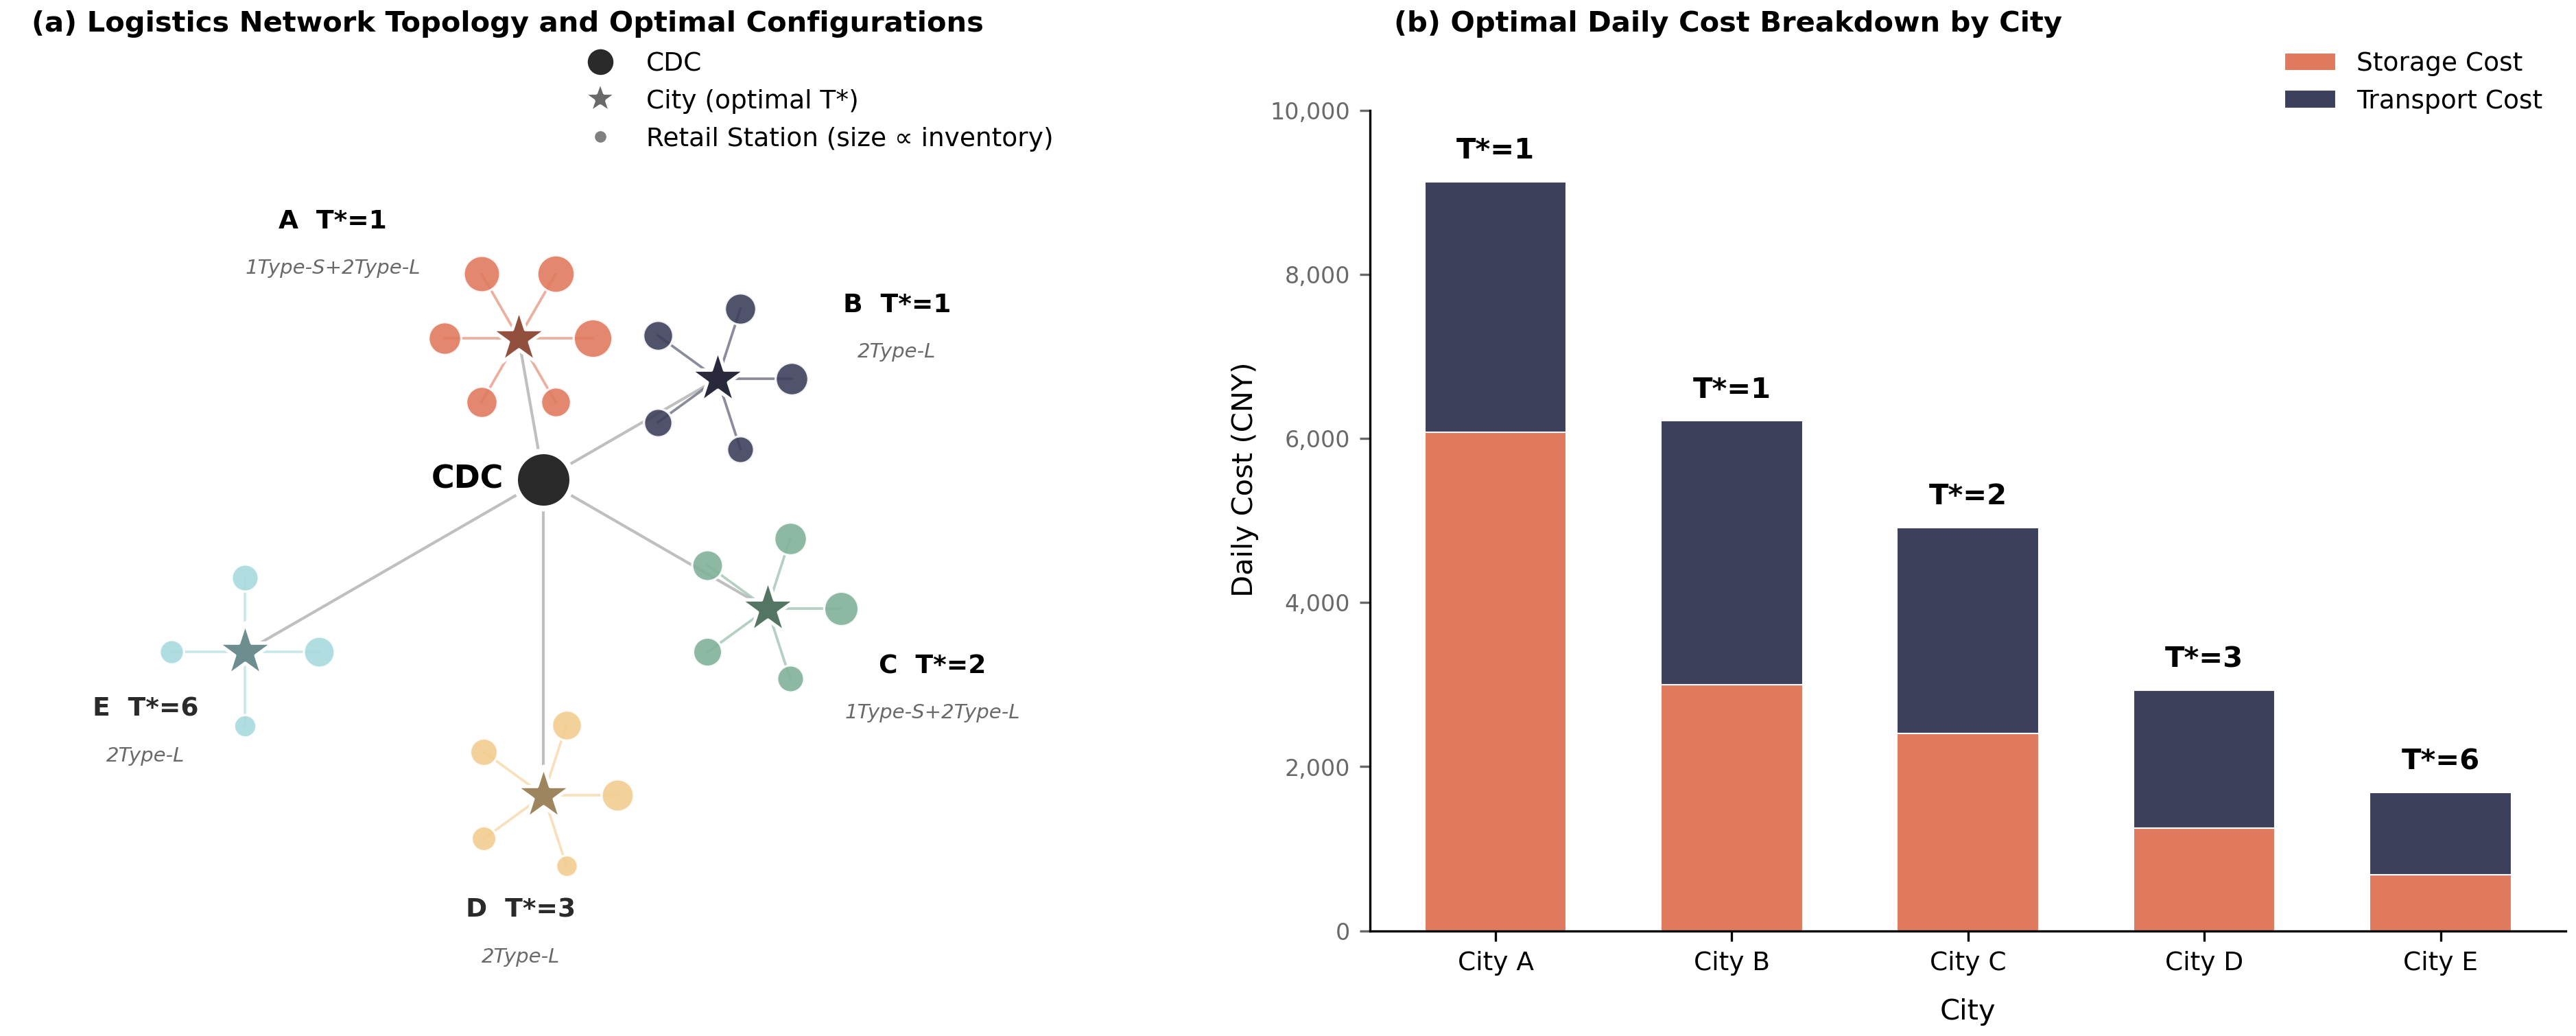
\includegraphics[width=\textwidth]{figures/combine_fig1_fig2.png}
    \caption{(a) 物流网络拓扑：1个CDC服务5个城市hub（A--E）。每个hub标注了其最优补货周期$T^*$和所需车辆数。(b) 各城市最优日成本分解，橙色为仓储成本，藏青色为运输成本。}
    \label{fig:topology}
\end{figure}

\section{城市级结果与敏感性分析}
\begin{table}[htbp]
\centering
\small
\caption{五个城市的最优配置与成本分解。}
\label{tab:city}
\begin{tabular}{@{}ccccccc@{}}
\toprule
城市 & $T^*$ & 站点数 & 车辆数 & 仓储成本(元) & 运输成本(元) & 总成本(元) \\
\midrule
A & 1 & 6 & 3 & 6,075.0 & 3,055.0 & 9,130.0 \\
B & 1 & 5 & 2 & 3,000.0 & 3,215.0 & 6,215.0 \\
C & 2 & 5 & 3 & 2,400.0 & 2,515.0 & 4,915.0 \\
D & 3 & 5 & 2 & 1,250.0 & 1,678.3 & 2,928.3 \\
E & 6 & 4 & 2 &   684.0 & 1,001.7 & 1,685.7 \\
\bottomrule
\end{tabular}
\end{table}

\subsection{敏感性分析}
图~\ref{fig:sensitivity}绘制了各城市在$T$从1到7天变化时的仓储、运输及总成本曲线。

\textbf{城市A和B}的总成本呈单调上升趋势。由于两者日需求量大，仓储成本$C_s(T)$几乎随$T$线性增长，并迅速压倒运输成本的有限节省。因此，最优周期为边界解$T^*=1$。

\textbf{城市C}呈现弱U型曲线，最小值位于$T^*=2$。在$T=1$时运输成本仍较高；将周期延长至2天所带来的运输节省恰好足以抵消额外的库存成本。

\textbf{城市D}展现出典型的U型曲线，内部最优点明确位于$T^*=3$。当$T<3$时运输惩罚严重；当$T>3$时，持有成本反弹并超过逐渐递减的运输节省。

\textbf{城市E}的需求量最小，因此可以承受最长的补货周期。总成本持续下降至$T^*=6$，之后$T=7$带来的库存增量使成本再次上升。

\begin{figure}[htbp]
    \centering
    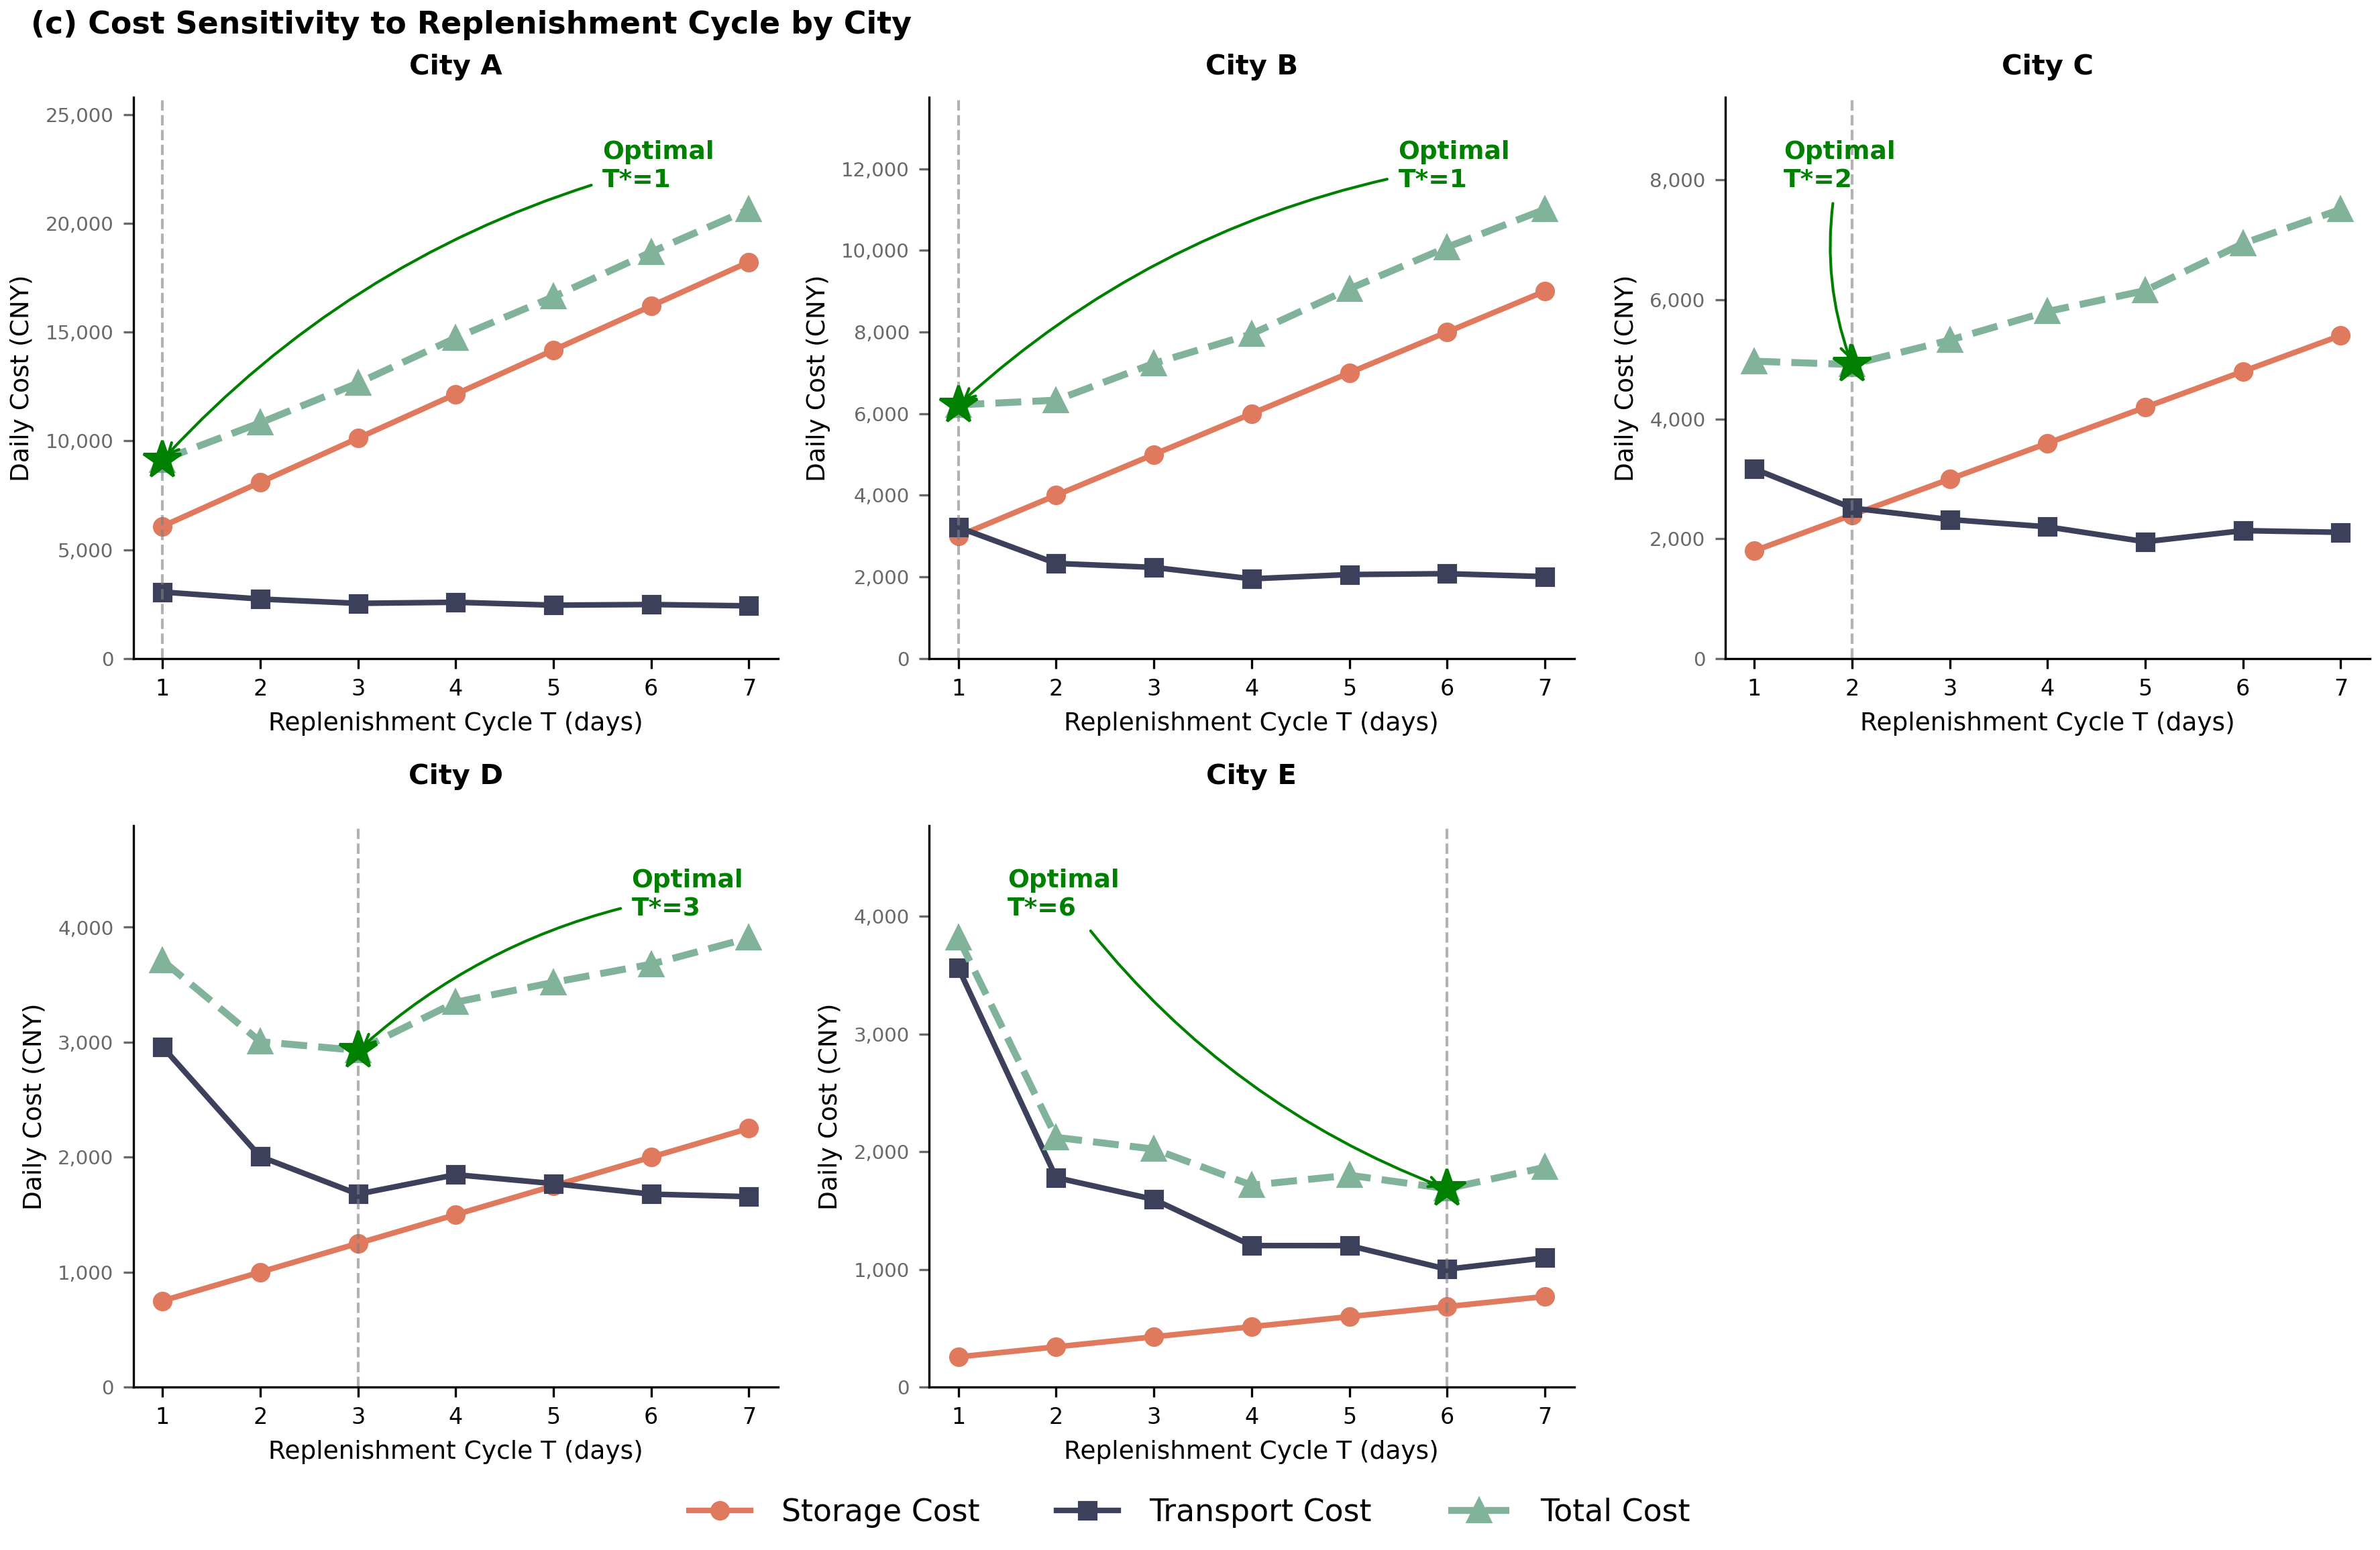
\includegraphics[width=0.95\textwidth]{figures/fix_fig3.png}
    \caption{五个城市对补货周期$T$的成本敏感性分析。绿色星标表示每个城市的最优$T^*$。}
    \label{fig:sensitivity}
\end{figure}

\section{全局优化与管理启示}
\subsection{系统层面表现}
全局最优解与各城市独立优化之和完全吻合：$T^*=\{A\!:\!1, B\!:\!1, C\!:\!2, D\!:\!3, E\!:\!6\}$，日均总成本为\textbf{24,874元}。尽管本实例中不存在协调惩罚，但全局枚举显示解空间的坡度较陡：前10优的替代方案仅比最优解高出30--145元/天（图~\ref{fig:global}左），印证了最优配置的稳健性。

更为重要的是，与统一$T$策略相比，\emph{差异化}的价值十分显著（图~\ref{fig:global}右）。强制所有城市采用$T=1$会使日成本增加2,968元（+11.9\%）；统一$T=3$增加5,290元（+21.3\%）；而统一$T=7$则使成本暴增20,058元（+80.6\%）。这些差距凸显了“一刀切”策略在异质网络中的经济不可接受性。

\begin{figure}[htbp]
    \centering
    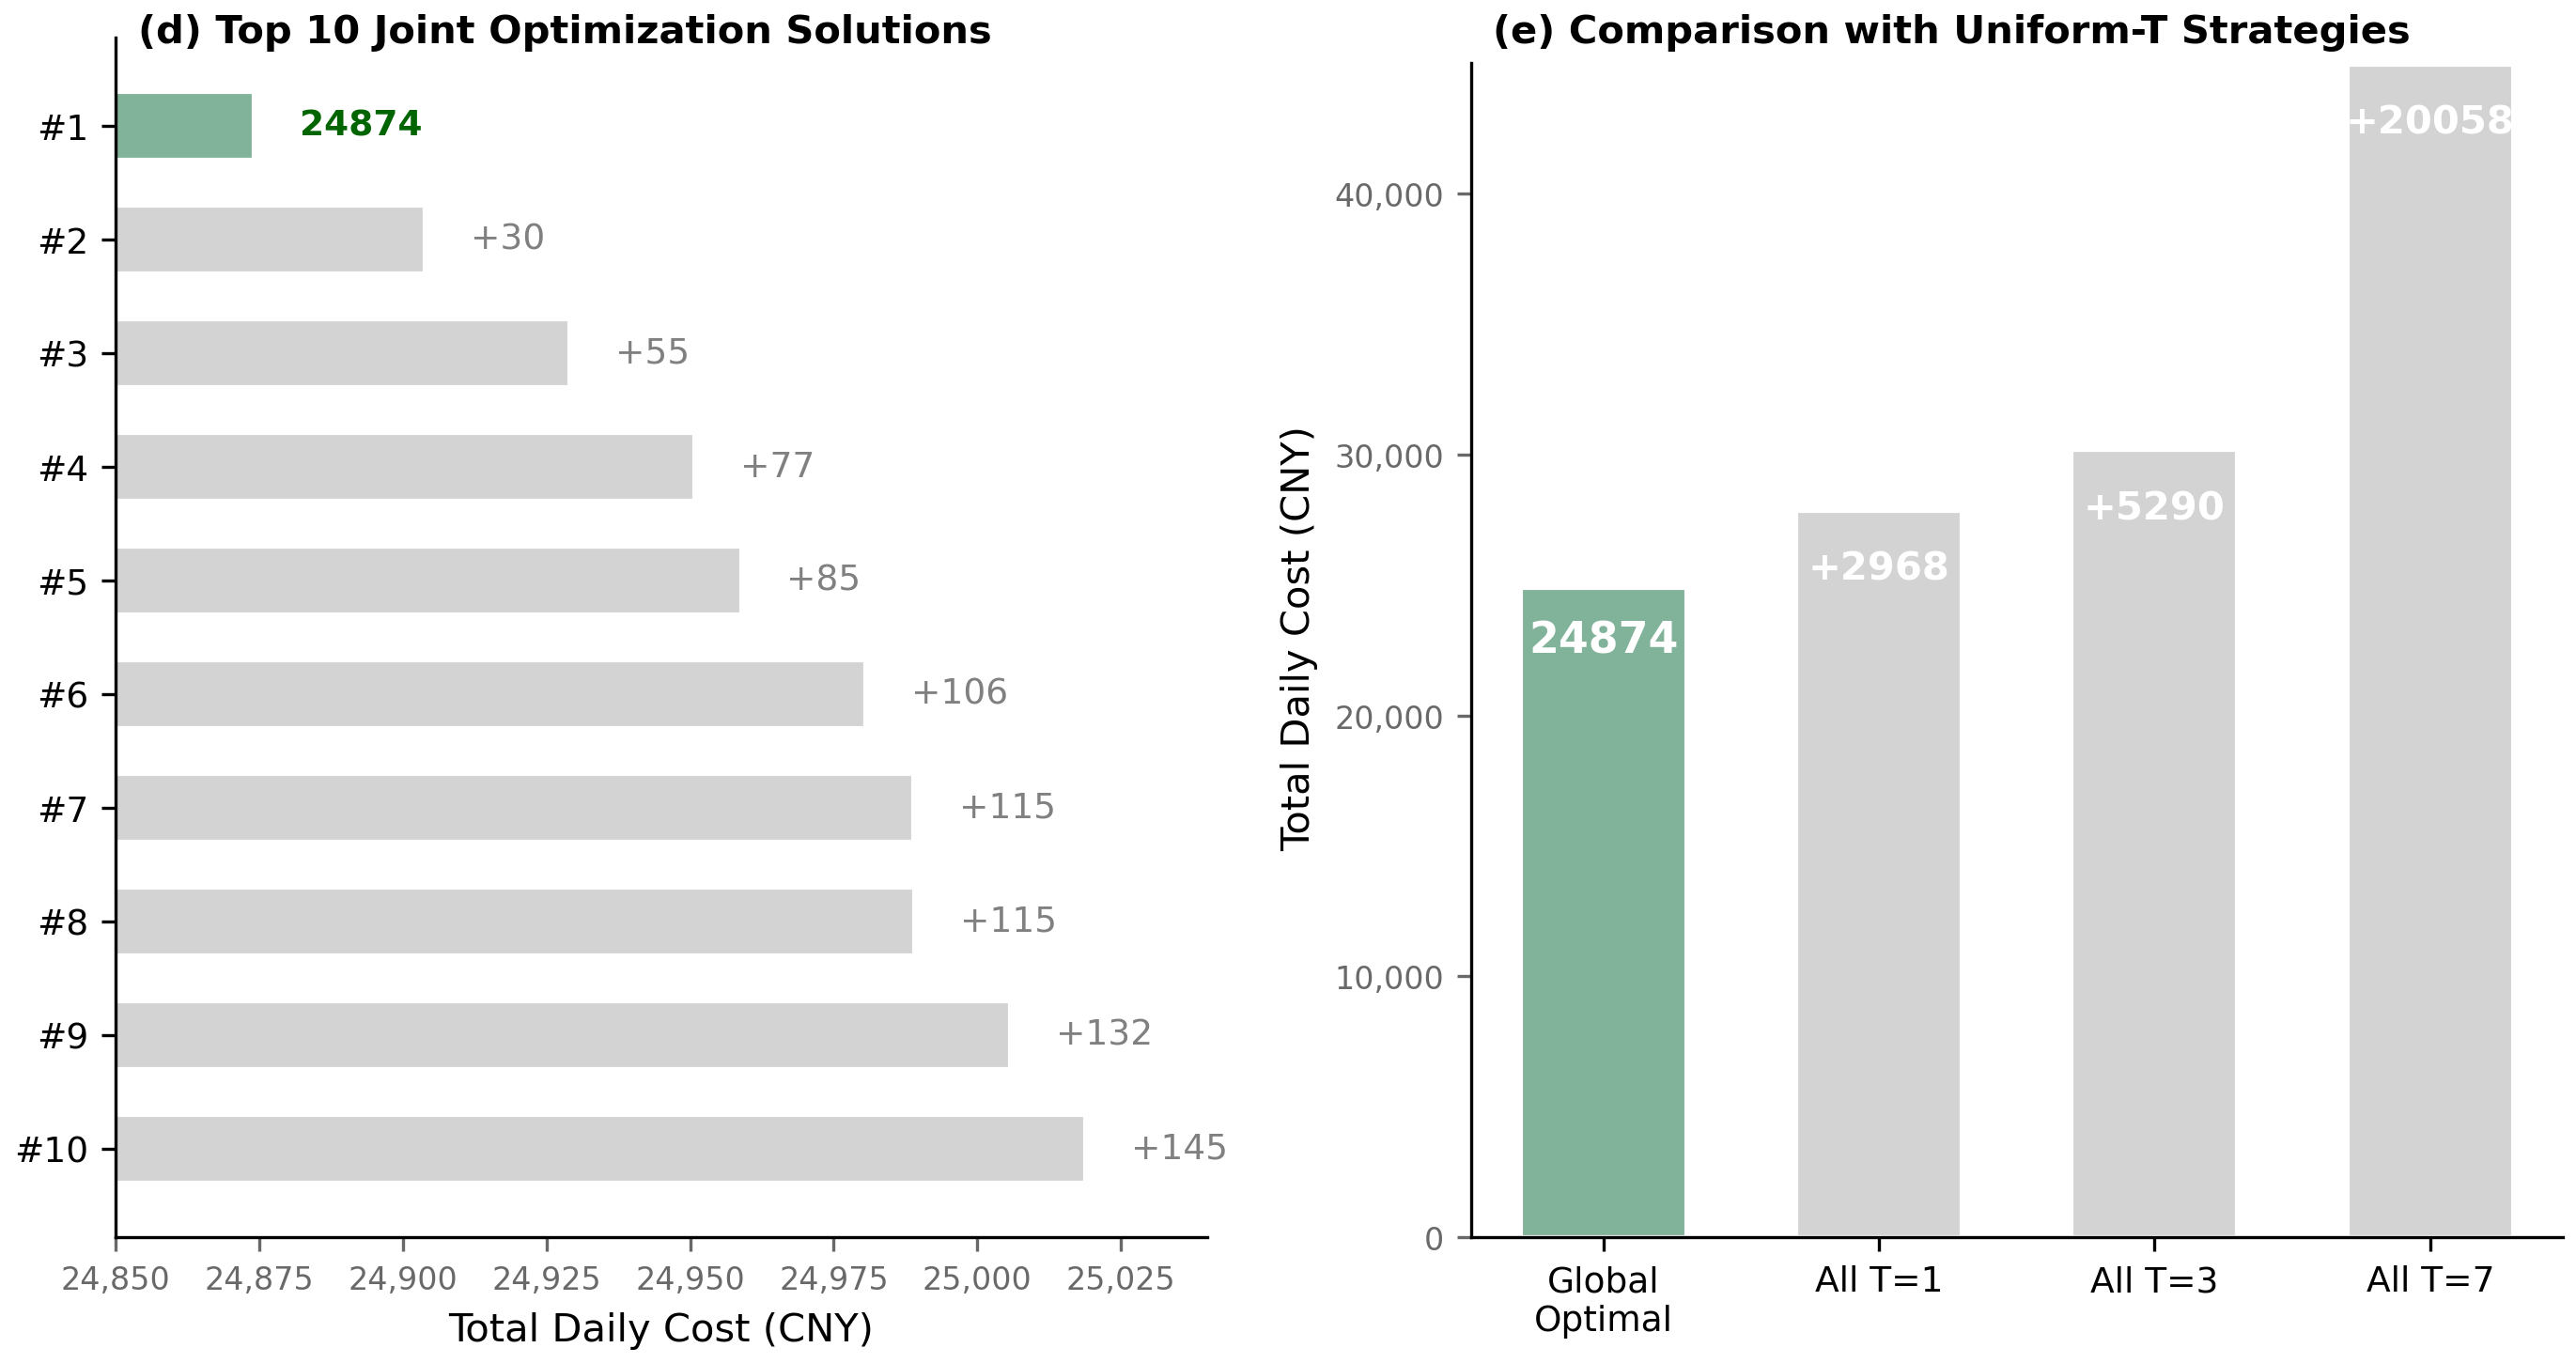
\includegraphics[width=\textwidth]{figures/fix_fig4.png}
    \caption{(左) 按日均总成本排序的前10个联合优化方案，最优解以绿色高亮显示。(右) 全局最优策略与统一$T$基线策略的对比，柱状图上方数字为相对于最优解的日均成本增量。}
    \label{fig:global}
\end{figure}

\subsection{管理启示}
我们为运营管理者提炼出四条可落地的建议：
\begin{enumerate}
    \item \textbf{拒绝统一策略。} 高需求城市（A、B）必须每日补货，而低需求城市（E）可以采用更长的周期。采用差异化的$T$政策是成本削减的最大杠杆。
    \item \textbf{关注仓储—运输拐点。} 对于中等需求城市如D，总成本曲线呈U型。精确校准拐点（本例中$T^*=3$）每天可节省数百元。
    \item \textbf{将车队规划与$T$联动。} 延长$T$会提高单次配送货量。管理者应同时审视是否需要更大车型或调整站点分组，以保持末端路径效率。
    \item \textbf{监控车辆装载率。} 低装载率意味着运力闲置和偏高的单位运输成本。对于利用率不足的车组（如$[B_4,B_5]$的$42.5\%$），管理者应考虑合并更多邻近站点或改用小车，以提升资产利用效率。
\end{enumerate}

\section{结论}
本文提出了一个可计算的多城生鲜物流联合库存—路径优化框架。通过结合城市级$T$优化与全局枚举，我们识别出一种差异化的补货策略，实现了24,874元/天的最低日均成本，并显著优于统一$T$基线。未来研究将扩展至随机需求与动态$T$调整，以进一步提升运营韧性。

\end{document}
